\newpage
\section{Porównanie detekcji źrenic}

Podobnie jak w pozostałych detekcjach, tak i w przypadku wykrywania źrenic algorytmy zostały porównane i wybrany jeden - najlepszy.

\subsection{Testowanie na statycznych zdjęciach}

\subsubsection{Oczekiwany wynik}

Oczekiwany rezultat detekcji źrenic został opisany dwoma parametrami:
\begin{itemize}
    \item \textbf{Środek źrenicy} - punkt kartezjański
    \item \textbf{Obszar tęczówki} - prostokątny obszar 
\end{itemize}

Przykładowe zdjęcie oka wraz z naniesionymi elementami pokazane jest na rysunku \ref{fig:expected_pupil}.


\begin{figure}[!h]
    \begin{center}
        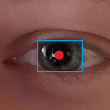
\includegraphics[scale=1.0]{img/pupil_section/pupil_expected.png}
        \caption{Przybliżona lokalizacja źrenicy i obszar tęczówki, które są oczekiwanym wynikiem algorytmu.}
        \label{fig:expected_pupil}
    \end{center}
\end{figure}

\subsubsection{Zbierane dane}

Podczas testów zbierane były następujące dane:

\begin{itemize}
    \item \textbf{W obszarze tęczówki} - ilość wykrytych punktów znajdujących się wewnątrz tęczówki oka
    \item \textbf{Poza obszarem tęczówki} - ilość wykrytych punktów znajdujących się poza tęczówką oka
    \item \textbf{Średni błąd} - średni błąd ze wszystkich detekcji (patrz Uwaga 1.)
    \item \textbf{Błąd <= 0.1} - ilość detekcji z~błędem nie większym niż $10\%$
    \item \textbf{Błąd <= 0.05} - ilość detekcji z~błędem nie większym niż $5\%$
\end{itemize}

\par

\textit{Uwaga 1.} Błąd (wykrycia punktu kartezjańskiego źrenicy) dla danego zdjęcia obliczany był następującym wzorem

\begin{align}
    b(P_1, P_2) = \frac{dist(P_1, P_2)}{hypot(w, h)} * 100\%
\end{align}

Gdzie:

\begin{itemize}
    \item \textbf{P\textsubscript{1}} - wykryty punkt
    \item \textbf{P\textsubscript{2}} - oczekiwany środek źrenicy
    \item \textbf{dist} - odległość między punktami (euklidesowa)
    \item \textbf{hypot} - przeciwprostokątna dla podanych przyprostokątnych (w przypadku regionu oka jest to przekątna)
    \item \textbf{w}, \textbf{h} - szerokość i~wysokość regionu oka
\end{itemize}



\subsubsection{Wybór funkcji projekcji}

Ze względu, że metoda PF może wykorzystywać różne funkcje projekcji do swojego działania konieczne było wyznaczenie i~wybranie najlepszej opcji. Badanie skuteczności przeprowadzone było dla następującego zestawu funkcji:

\begin{itemize}
    \item Całkowa
    \item Wariancja kwadratowa
    \item Wariancja pierwiastkowa
    \item Wariancja liniowa
    \item Ogólna z~wariancją kwadratową
    \item Ogólna z~wariancją pierwiastkową
    \item Ogólna z~wariancją liniową
\end{itemize}

W~przypadku funkcji ogólnej dodatkowo zostało przeprowadzone przeszukiwanie celem ustalenia najlepszego współczynnika $\alpha$ dla poszczególnych opcji. Badana była wielkość tego parametru w~przedziale $[0.01, 0.99]$ ze skokiem $0.01$ (wykluczono wartości $0.00$ oraz $1.00$, ponieważ odpowiadają one odpowiednio funkcji całkowej i~funkcji wariancji).

\par

Finalnie najlepsze w~poszczególnych wariantach okazały się następujące wartości współczynnika $\alpha$:

\begin{itemize}
    \item Ogólna z~wariancją kwadratową: $0.99$
    \item Ogólna z~wariancją pierwiastkową: $0.01$
    \item Ogólna z~wariancją liniową: $0.31$
\end{itemize}

W przypadku funkcji ogólnej z~wariancją kwadratową najlepszy rezultat dał parametr $\alpha=0.99$, co w~przybliżeniu degeneruje ją do wariancji kwadratowej. Natomiast w~przypadku pierwiastkowej ($\alpha=0.01$) do funkcji całkowej. Potwierdzają to również wyniki w~tabeli~\ref{tab:eye_pupil_projection_accuracy_result}, gdzie opisane przypadki osiągają takie same lub zbliżone rezultaty.

\begin{table}[!h]

\centering
\caption{Skuteczność algorytmu PF zależnie od funkcji projekcji na zbiorze danych}
\label{tab:eye_pupil_projection_accuracy_result}
\begin{tabular}{|c|c|c|c|c|c|}
\hline
 &
  \textbf{\begin{tabular}[c]{@{}c@{}}W obszarze \\ tęczówki \end{tabular}} &
  \textbf{\begin{tabular}[c]{@{}c@{}}Poza obszarem \\ tęczówki \end{tabular}} &
  \textbf{\begin{tabular}[c]{@{}c@{}}Średni \\ błąd\end{tabular}} &
  \textbf{\begin{tabular}[c]{@{}c@{}}Błąd \\ <= 0.1\end{tabular}} &
  \textbf{\begin{tabular}[c]{@{}c@{}}Błąd \\ <= 0.5\end{tabular}}
  \\ \hline \hline

\textbf{Całkowa} &
  85 &
  51 &
  14,35\% &
  53 &
  26  \\ \hline
  
\textbf{Wariancji, kwadratowa} &
  98 &
  38 &
  13,51\% &
  60 &
  27 
  \\ \hline
  
\textbf{Wariancji, pierwiastkowa} &
  79 &
  57 &
  14,66\% &
  47 &
  29  \\ \hline
  
  \textbf{Wariancji, liniowa} &
  51 &
  85 &
  23,12\% &
  24 &
  4  \\ \hline
  
  \textbf{Ogólna, kwadratowa} &
  98 &
  38 &
  13,51\% &
  60 &
  27 
  \\ \hline
  
\textbf{Ogólna, pierwiastkowa} &
  85 &
  51 &
  14,27\% &
  53 &
  26  \\ \hline
  
  \textbf{Ogólna, liniowa} &
  86 &
  50 &
  14,17\% &
  53 &
  26  \\ \hline
  
  \hline
\end{tabular}%
\end{table}

Najlepszą skuteczność wykazały funkcje wariancji kwadratowej oraz ogólna kwadratowa. Wykryły one najwięcej punktów wewnątrz tęczówki - $72\%$ oraz uzyskały najmniejszy średni błąd - $13.51\%$. Ze względu na opisaną wyżej degradacje, której przyczyną jest współczynnik $\alpha$ z~tej pary wybrana została funkcja wariancji, która musi wykonać mniej obliczeń w~czasie swojego działania. Dlatego ta wersja funkcji była wykorzystywana w~dalszej części badań.

\subsubsection{Badanie skuteczności detekcji}






\begin{table}[!h]
\label{tab:eye_pupil_detection_accuracy_result}
\centering
\caption{Skuteczność algorytmów detekcji źrenic na zbiorze danych}
\begin{tabular}{|c|c|c|c|c|c|}
\hline
 &
  \textbf{\begin{tabular}[c]{@{}c@{}}W obszarze \\ tęczówki \end{tabular}} &
  \textbf{\begin{tabular}[c]{@{}c@{}}Poza obszarem \\ tęczówki \end{tabular}} &
  \textbf{\begin{tabular}[c]{@{}c@{}}Średni \\ błąd\end{tabular}} &
  \textbf{\begin{tabular}[c]{@{}c@{}}Błąd \\ <= 0.1\end{tabular}} &
  \textbf{\begin{tabular}[c]{@{}c@{}}Błąd \\ <= 0.5\end{tabular}}
  \\ \hline \hline

\textbf{CDF} &
  113 &
  23 &
  10,72\% &
  87 &
  54  \\ \hline
  
\textbf{PF} &
  98 &
  38 &
  13,51\% &
  60 &
  27 
  \\ \hline
  
\textbf{EA} &
  68 &
  68 &
  19,68\% &
  42 &
  14  \\ \hline
  
  \hline
\end{tabular}%
\end{table}


W przypadku progowania przy pomocy dystrybuanty na prawidłową detekcje wpływ miała jakość wycinka zdjęcia podawanego na wejście metody. W~przypadku gdy duża była jego ostrość, a~oko zajmowało subiektywnie duży obszar to algorytm radził sobie bardzo dobrze. Metoda uzyskiwała dobre wyniki zarówno w~przypadku gdy tęczówka oka była ciemna, jak i~jasna. Negatywny wpływ na skuteczność detekcji miało występowanie na wycinku zdjęcia brwi, a~w~szczególności gdy były one w~ciemnym odcieniu lub nałożony był na nie mocny makijaż. Podobnie intensywna barwa rzęs skutkowała obniżeniem dokładności wskazywania lokalizacji źrenicy. Lepsze rezultaty metoda uzyskiwała gdy na wycinku znajdowała się tylko i~wyłącznie gałka oczna. W~przypadku gdy źrenica miała jasny odcień wynikający np. z~dużego natężenia padającego światła to uzyskiwane rezultaty nie były zadowalające. Jeśli algorytmowi udało się wskazać punkt należący do tęczówki, to w~większości przypadków wynikiem był jej środek oraz źrenica. W~ogólności, skuteczność tej metody opierała się w~dużej mierze na występowaniu ciemnych punktów innych niż tęczówka i~źrenica.

\par

Metoda projekcji lepsze rezultaty detekcji wykazywała na obszarach oczu o~małym kontraście i~ostrości. Gorsza jakość zdjęć miała pozytywny wpływ na jej działanie. Częstym zjawiskiem było wskazanie tylko jednej składowej poprawnie - poziomej lub pionowej. Algorytm ten w~części przypadków wskazywał rzęsy zamiast źrenic. Prawidłowe detekcje występowały przy bardzo wyraźnych przejściach między białą częścią oka, a~tęczówką. Jeśli region źrenicy był ciemniejszy niż reszta obszaru oka to detekcja uzyskiwała lepsze rezultaty. Występowanie ramek okularów przeszkadzało w~prawidłowym wskazaniu szukanego punktu.

\par

Analiza krawędzi całkowicie nie radziła sobie z~detekcją w~przypadku gdy występowało dużo wyraźnych konturów innych niż tęczówka lub źrenica. Dobre rezultaty osiągane były jeśli obszar oka był jasny i~naświetlony. W~przeciwieństwie do projekcji metoda ta lepiej radziła sobie przy wycinkach dobrej jakości i~o dużej ostrości. Porównując ten algorytm do dwóch pozostałych jego zachowanie wydawało się dużo bardziej losowe, ponieważ w~wielu przypadkach trudno było wskazać powody zwróconej złej lokalizacji. Wyniki procentowe jak i~subiektywne odczucia wskazują jednoznacznie, że metoda oparta na analizie krawędzi radziła sobie znacznie najgorzej.





\subsubsection{Badanie szybkości detekcji} \label{section:test_pupil_speed_img}

\begin{table}[!h]
\label{tab:eye_pupil_speed}
\centering
\caption{Czas przetwarzania algorytmów detekcji źrenic na zbiorze danych}

\begin{tabular}{|c|c|c|c|}
\hline
 & 
  \textbf{\begin{tabular}[c]{@{}c@{}}Całkowity czas \\ przetwarzania \end{tabular}} &
  \textbf{\begin{tabular}[c]{@{}c@{}}Średni czas\\ przetwarzania \\ pojedynczej iteracji\end{tabular}} &
  \textbf{\begin{tabular}[c]{@{}c@{}}Średni czas\\przetwarzania \\ pojedynczego\\zdjęcia\end{tabular}} \\ \hline\hline
  
\textbf{PF} & 
  0,272 s &
  0,00272 s &
  0,00002001 s    \\ \hline
  
\textbf{EA} & 
  0,765 s &
  0,00765 s &
  0,00005627 s  \\ \hline
  
\textbf{CDF} & 
  0,637 s &
  0,00637 s &
  0,00004684 s \\ \hline

  \hline
\end{tabular}%

\end{table}

Najszybszym okazał się algorytm oparty na funkcji projekcji. Przetworzenie jednego wycinka oka zajęło mu średnio $2.0*10^{-5}s$. Dwukrotnie dłużej trwało wykonanie metody z~użyciem progowania opartego o~dystrybuantę. Najwolniej natomiast działała analiza krawędzi uzyskując czas $5.6*10^{-5}$.

\par

Wyniki zdają się oddawać naturę poszczególnych metod, ponieważ projekcja wymaga maksymalnie dwóch przejść całej macierzy obrazu. Natomiast algorytm oparty na analizie krawędzi wykorzystuje filtry oraz metodę Canny, dlatego ma największą złożoność czasową.

\par

Wszystkie metody są bardzo szybkie (rząd wielkości $10^{-5}s$) i~nawet najwolniejsza z~nich mogłaby być wykonana prawie 18 tyś. razy na sekundę. Przekłada się to na zerowe obciążenie całej aplikacji, która wykrywając jedynie twarz osiąga raptem $16$ klatek na sekundę dla barw RGB (rozdział~\ref{section:face_speed_live}). Z~tego powodu podczas wyboru najlepszego algorytmu detekcji źrenic nie była brana pod uwagę szybkość poszczególnych metod, a~jedynie ich skuteczność.




\subsection{Testowanie na obrazie z~kamery}

Przetestowanie skuteczności detekcji na obrazie z~kamery i~przedstawienie ich w~postaci liczbowej byłoby bardzo trudne. Z~tego powodu algorytm został przebadany poprzez obserwacje zachowania detekcji na podglądzie na żywo. Testy były przeprowadzone w~takich samych warunkach jak pozostałe elementy systemu. Wyniki są subiektywnym odczuciem autora projektu i~przedstawione w~formie opisowej. 

\par

Ze względu na wyniki szybkościowe detekcji źrenic (rozdział~\ref{section:test_pupil_speed_img}), które jednoznacznie wykazały marginalny czas przetwarzania wszystkich algorytmów, testy czasowe na obrazie z~kamery na żywo zostały uznane za niepotrzebne i~pominięte.

\subsubsection{Badanie skuteczność detekcji}

Podobnie jak w~testach przeprowadzonych na statycznych zdjęciach algorytm CDF uzyskał subiektywnie najlepsze rezultaty. We wszystkich scenariuszach sprawdził się wystarczająco. Nawet w~momencie gdy nie wykrywał dobrze środka źrenicy to wskazania znajdowały się w~obszarze tęczówki. Pracował stabilnie zarówno w~centralnym położeniu oka jak i~przy wzroku zwróconym w~bok. 

\par 

Algorytm PF radził sobie dobrze tylko połowicznie. Najlepsze rezultaty osiągnął w~przypadku światła padającego zza użytkownika. Wtedy zarówno centralne jak i~boczne położenie był prawidłowo wykrywane. W~pozostałych badaniach dobre wyniki osiągał gdy oczy był skierowane w~bok, a~w~przypadku spojrzenia wprost przed siebie lokalizacja podawana była chaotycznie. Test w~ciemnym pomieszczeniu potwierdził, że metoda dobrze radzi sobie przy małym kontraście i~jasności. 

\par

Analiza krawędzi w~przypadku obrazu na żywo w~ogóle się nie sprawdziła. W~żadnych warunkach detekcja nie była wystarczająca na potrzeby pracy dyplomowej. Przez większość czasu zwracaną lokalizacją były rogi obszaru oczu.


 

\subsection{Wybór algorytmu detekcji źrenic}

Najskuteczniejsza okazała się metoda oparta na progowaniu z~użyciem dystrybuanty. W~teście na zbiorze danych~$83\%$ wykrytych punktów znajdowało się wewnątrz tęczówki. Subiektywnie, najlepsze i~wystarczające rezultaty uzyskała również w~badaniu obrazu na żywo z~kamery.

\par

Szybkość wszystkich algorytmów stała na tak wysokim i~marginalnym poziomie, że nie była brana jako czynnik wpływający na wybór algorytmu.

\par

Z powodu wykrywalności źrenic rozwiązanie CDF zostało wybrane jako najlepsze i podstawowe w~projekcie.